\documentclass{article}
\setlength{\parskip}{5pt} % esp. entre párrafos
\setlength{\parindent}{0pt} % esp. al inicio de un párrafo
\usepackage{amsmath} % mates
\usepackage{url} % que las URLs se vean lindos
\usepackage[top=25mm,left=20mm,right=20mm,bottom=25mm]{geometry} % márgenes
\usepackage{parskip}
\usepackage[utf8]{inputenc}
\usepackage{amsmath,amsfonts,amssymb,mathtools}
\usepackage{graphicx,float}
\usepackage{algorithmic}
\usepackage{minted}
\usepackage{subcaption}
\usepackage{multicol}
\usepackage{listings}
\usepackage{xcolor}
\usepackage[sort&compress,numbers]{natbib} % referencias
\usepackage{minted}
\usepackage{hyperref} % ligas de URLs
\usepackage{graphicx} % poner figuras
\usepackage[spanish]{babel} % otros idiomas
\usepackage{listings}
\author{Raul L.} % author
\title{Pr\'{a}ctica 10: algoritmo genético} %título
\date{\today}
\begin{document} % inicia contenido

\maketitle % cabecera


\section{Introducci\'{o}n}\label{intro} % sección y etiqueta
El problema de la mochila (inglés: knapsack) es un problema clásico de optimización, particularmente de programación entera, donde la tarea consiste en seleccionar un subconjunto de objetos de tal forma que (i) no se exceda la capacidad de la mochila en términos de la suma de los pesos de los objetos incluidos, y que (ii) el valor total de los objetos incluidos sea lo máximo posible. Este problema es pseudo-polinomial ya que existe un algoritmo de tabulación que determina la combinación óptima.
Aunque el algoritmo pseudo-polinomial sirve solamente para pesos enteros, nos servirá para esta décima práctica, donde probamos la implementación de un algoritmo genético en R de manera paralela. Los algoritmos genéticos se suelen utilizar en casos donde no existe ningún algoritmo exacto eficiente, pero para fines de aprendizaje, nos conviene comparar qué tan cerca a la solución óptima (que nos da el algoritmo pseudo-polinomial) logramos llegar con un algoritmo genético.

Un algoritmo genético representa posibles soluciones a un problema en términos de un genoma que en nuestro caso va a ser un vector de verdades y falsos, indicando cuáles objetos vamos a incluir en la mochila (TRUE o 1 significa que llevamos el objeto, FALSE o 0 que lo descartamos de la selección).

Preparamos algunas subrutinas necesarias:

verificar si una selección particular respeta la capacidad de la mochila o no;
calcular el valor total de los objetos incluidos;
generar una selección uniformemente al azar;
generar pesos enteros y ordenados al azar (normalmente distribuidos);
asignar a cada objeto un valor al azar (normalmente distribuidos alrededor de los pesos pero con desviación estándar uniformemente distribuidos)\citep{2}.


\section{Objetivo}
Genere tres instancias con tres distintas reglas (nueve en total):

el peso y el valor de cada objeto se generan independientemente con una distribución uniforme,
el valor de cada objeto se generan independientemente con una distribución exponencial y su peso es inversamente correlacionado con el valor,
el peso de cada objeto se generan independientemente con una distribución normal y su valor es (positivamente) correlacionado con el cuadrado del peso, con un ruido normalmente distribuido de baja magnitud.
Determina para cada uno de los tres casos si variar la probabilidad de mutación, la cantidad de cruzamientos y el tamaño de la población (dos o tres niveles basta) tienen un efecto (solo o en combinación) estadísticamente significativo (usando por lo menos tres réplicas por instancia) en la calidad de resultado, manteniendo el tiempo de ejecución fijo\citep{2}.


\section{C\'{o}digo}
Para este código se utilizó como base el código de la doctora donde se agregaron las 3 reglas.


 Código en Python 
\url{https://github.com/satuelisa/Simulation/blob/master/Particles/creation.py}
\newpage
{\bf Código creado en Python}

\url{https://github.com/Raullr28/Resultados/tree/main/P_10}

\renewcommand{\listingscaption}{Código}

\begin{listing}[H]
\begin{minted}{python}

for regla in range(3):
    print("############## regla:",regla,"#################")
    if regla == 0:
        pesos = pesos1(n, 15, 80)
        valores = valores1(pesos, 10, 500)
    if regla == 1:
        valores = valores2(n, 10, 500)
        pesos = pesos2(valores, 15, 80)
    if regla == 2:
        pesos = pesos3(n, 15, 80)
        valores = valores3(pesos, 10, 500)

  \end{minted}
  \label{lst:fibo}
  \caption{Representación de las 3 reglas generadas.}
  
  
\end{listing}
\renewcommand{\listingscaption}{Código}
\begin{listing}[H]

\begin{minted}{python}

def pesos1(cuantos, low, high):
    return np.round(normalizar(np.random.uniform(size = cuantos)) * (high - low) + low)
 
def valores1(pesos, low, high):
    n = len(pesos)
    valores = np.empty((n))
    for i in range(n):
        valores[i] = np.random.uniform(pesos[i], random(), 1)
    return normalizar(valores) * (high - low) + low

def pesos2(valores, low, high):
    cuantos=1/valores
    return np.round(normalizar(cuantos) * (high - low) + low)
 
def valores2(cuantos, low, high):
    valores = expon.rvs(size= cuantos)
    return normalizar(valores) * (high - low) + low

def pesos3(cuantos, low, high):
    return np.round(normalizar(np.random.normal(size = cuantos)) * (high - low) + low)
 
def valores3(pesos, low, high):
    n = len(pesos)
    valores = np.empty((n))
    magnitud=0.1
    ruido=np.random.normal(loc=5, size = n)
    ruido=ruido*magnitud
    for i in range(n):
        valores[i] = (pesos[i]**2)+ ruido[i]
    return normalizar(valores) * (high - low) + low
    
\end{minted}
\label{lst:fibo}
\caption{Representación ciclo de la partícula.}
\end{listing}

\renewcommand{\listingscaption}{Código}
\begin{listing}[H]

\begin{minted}{python}

def poblacion_inicial(n, tam):
    pobl = np.zeros((tam, n))
    for i in range(tam):
        pobl[i] = (np.round(np.random.uniform(size = n))).astype(int)
    return pobl
 
def mutacion(sol, n):
    pos = randint(0, n - 1)
    mut = np.copy(sol)
    mut[pos] = 1 if sol[pos] == 0 else 0
    return mut
  
def reproduccion(x, y, n):
    pos = randint(2, n - 2)
    xy = np.concatenate([x[:pos], y[pos:]])
    yx = np.concatenate([y[:pos], x[pos:]])
    return (xy, yx)
    
  \end{minted}
  \label{lst:fibo}
  \caption{Representación ciclo de la partícula.}
\end{listing}




\newpage
% Computational Results
\section{Resultados}
En una gráfica de barras se graficó los resultados del comportamiento del tiempo con las diferentes instancias obtenidas, se agregó una gráfica de violines para saber con que instancia se obtiene un pequeño porcentaje.


%%%%%%%%%%%%%%%%%%%%% imagen 1
\begin{figure}[H]
\centering
\begin{subfigure}[b]{1.0\linewidth}
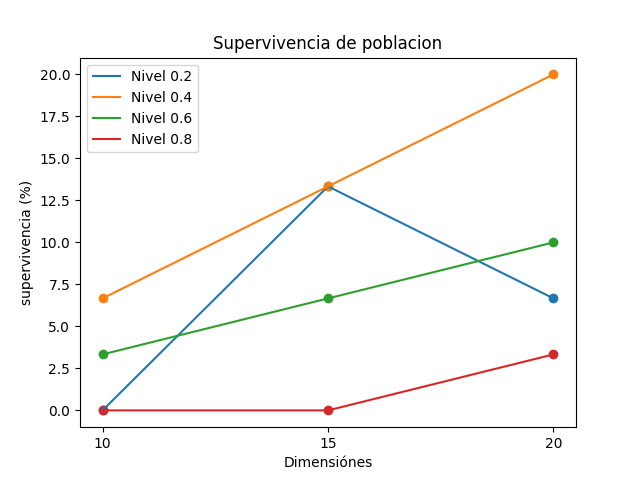
\includegraphics[width=\linewidth]{imagenes/Figure_1.png}
\end{subfigure}
\caption{Gráfica de tiempo de ejecución.}
\label{fig:westminster}
\end{figure}
%%%%%%%%%%%%%%%%%%%%%%%  final 


%%%%%%%%%%%%%%%%%%%%% imagen 2
\begin{figure}[H]
\centering
\begin{subfigure}[b]{1.0\linewidth}
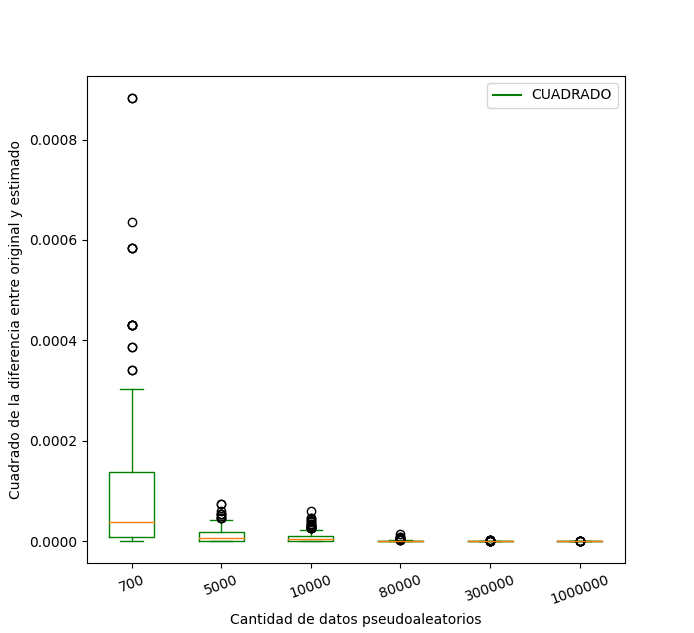
\includegraphics[width=\linewidth]{imagenes/Figure_2.png}
\end{subfigure}
\caption{Grafica de Porcentaje.}
\label{fig:westminster}
\end{figure}
%%%%%%%%%%%%%%%%%%%%%%%  final 



%%%%%%%%%%%%%%%%%%%%% imagen 3
\begin{figure}[H]
\centering
\begin{subfigure}[b]{1.0\linewidth}
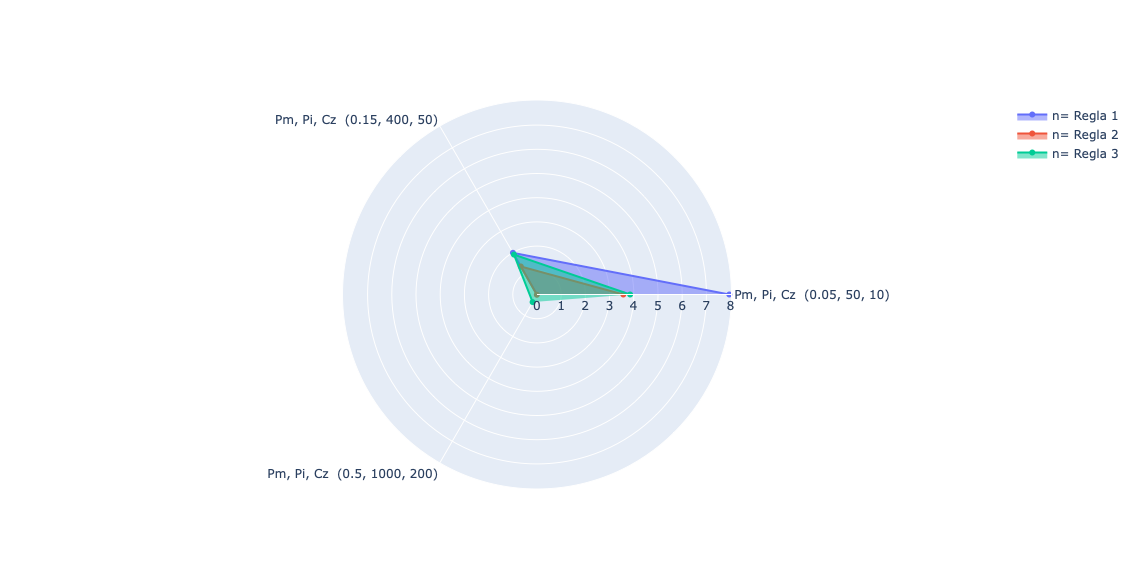
\includegraphics[width=\linewidth]{imagenes/newplot.png}
\end{subfigure}
\caption{Grafica de reglas.}
\label{fig:westminster}
\end{figure}
%%%%%%%%%%%%%%%%%%%%%%%  final 

\newpage
\section{Reto 1}
Como un primer reto, cambia la selección de mutación y de los padres para reproducción a que use selección de ruleta: cada solución se selecciona como padre con una probabilidad que es linealmente proporcional a su valor de función objetivo y a su factibilidad, combinando los dos a alguna función que parezca conveniente e inversamente proporcional a alguna combinación de factibilidad y objectivo para la mutación (recomiendo aprovechar el parámetro prob en sample).

Aplicar la selección de ruleta a las fases de cruzamiento y de supervivencia: en vez de quedarnos con las mejores soluciones, cada solución tiene una probabolidad de entrar a la siguiente generación que es proporcional a su valor de la función objetivo, incorporando el sí o no es factible la solución en cuestión, permitiendo que los $k$ mejores entre las factibles entren siempre (donde $k$ es un parámetro). Estudia nuevamente el efecto de este cambio en la calidad de la solución en los tres casos\citep{2}.

%%%%%%%%%%%%%%%%%%%%% imagen 1
\begin{figure}[H]
\centering
\begin{subfigure}[b]{1.0\linewidth}
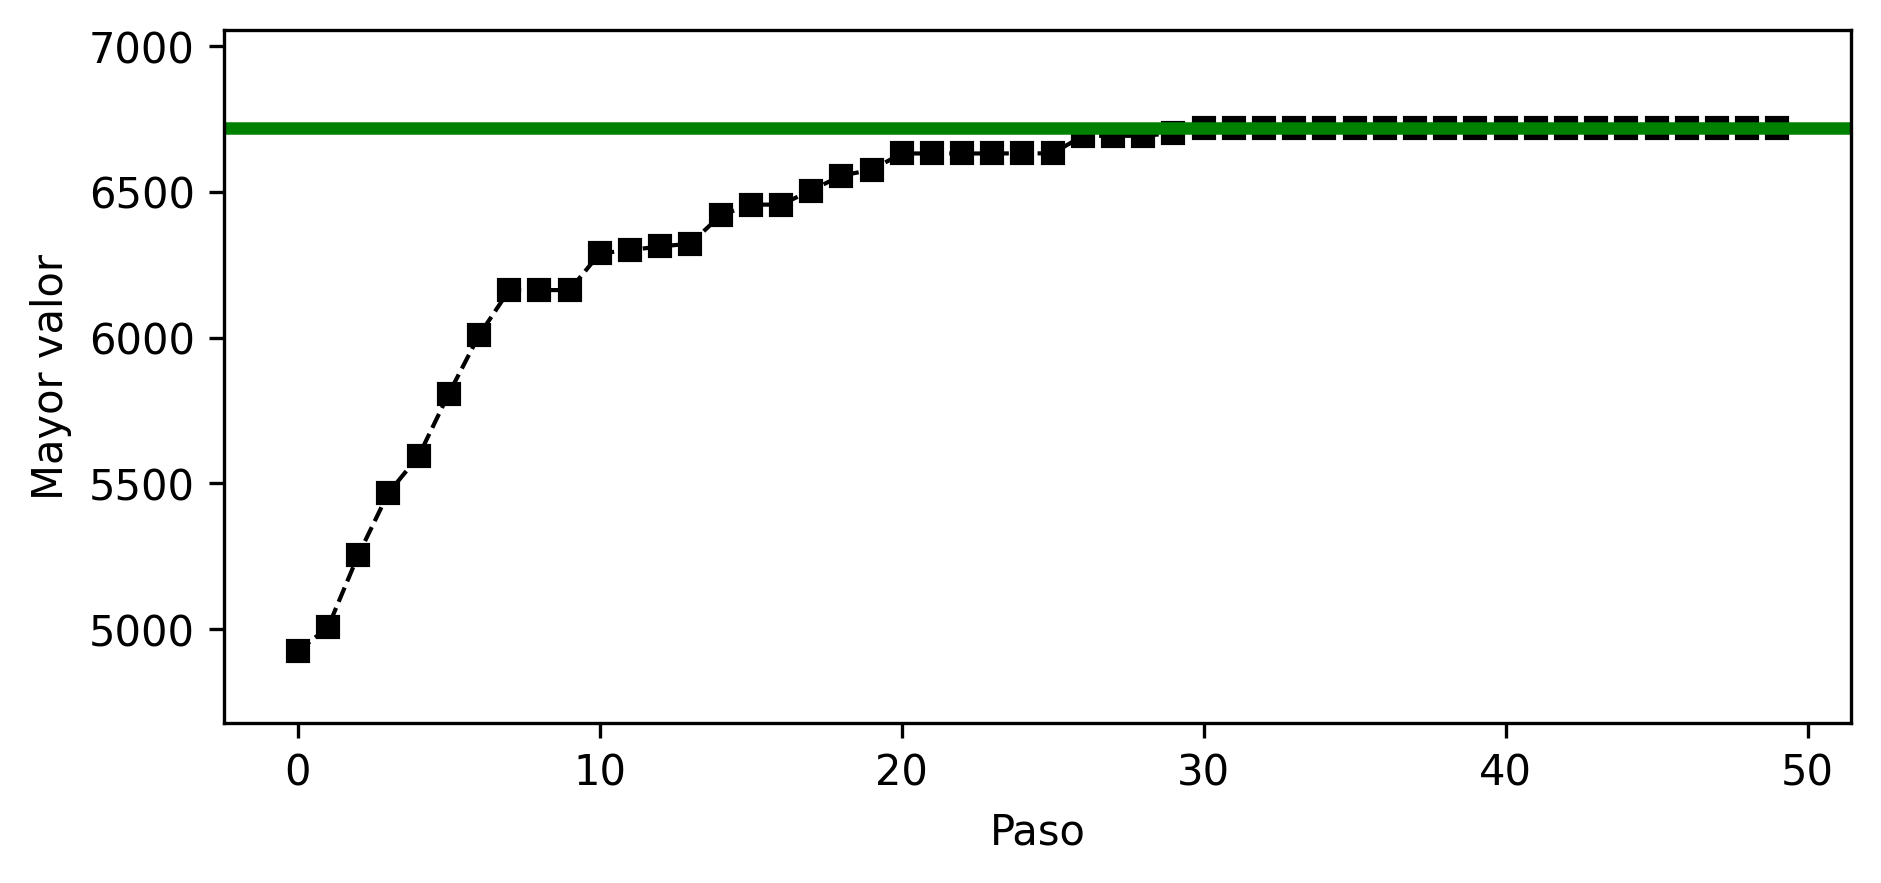
\includegraphics[width=\linewidth]{imagenes/figura_rp2.png}
\end{subfigure}
\caption{Gráfica de comportamiento regla 1.}
\label{fig:westminster}
\end{figure}
%%%%%%%%%%%%%%%%%%%%%%%  final 


%%%%%%%%%%%%%%%%%%%%% imagen 2
\begin{figure}[H]
\centering
\begin{subfigure}[b]{1.0\linewidth}
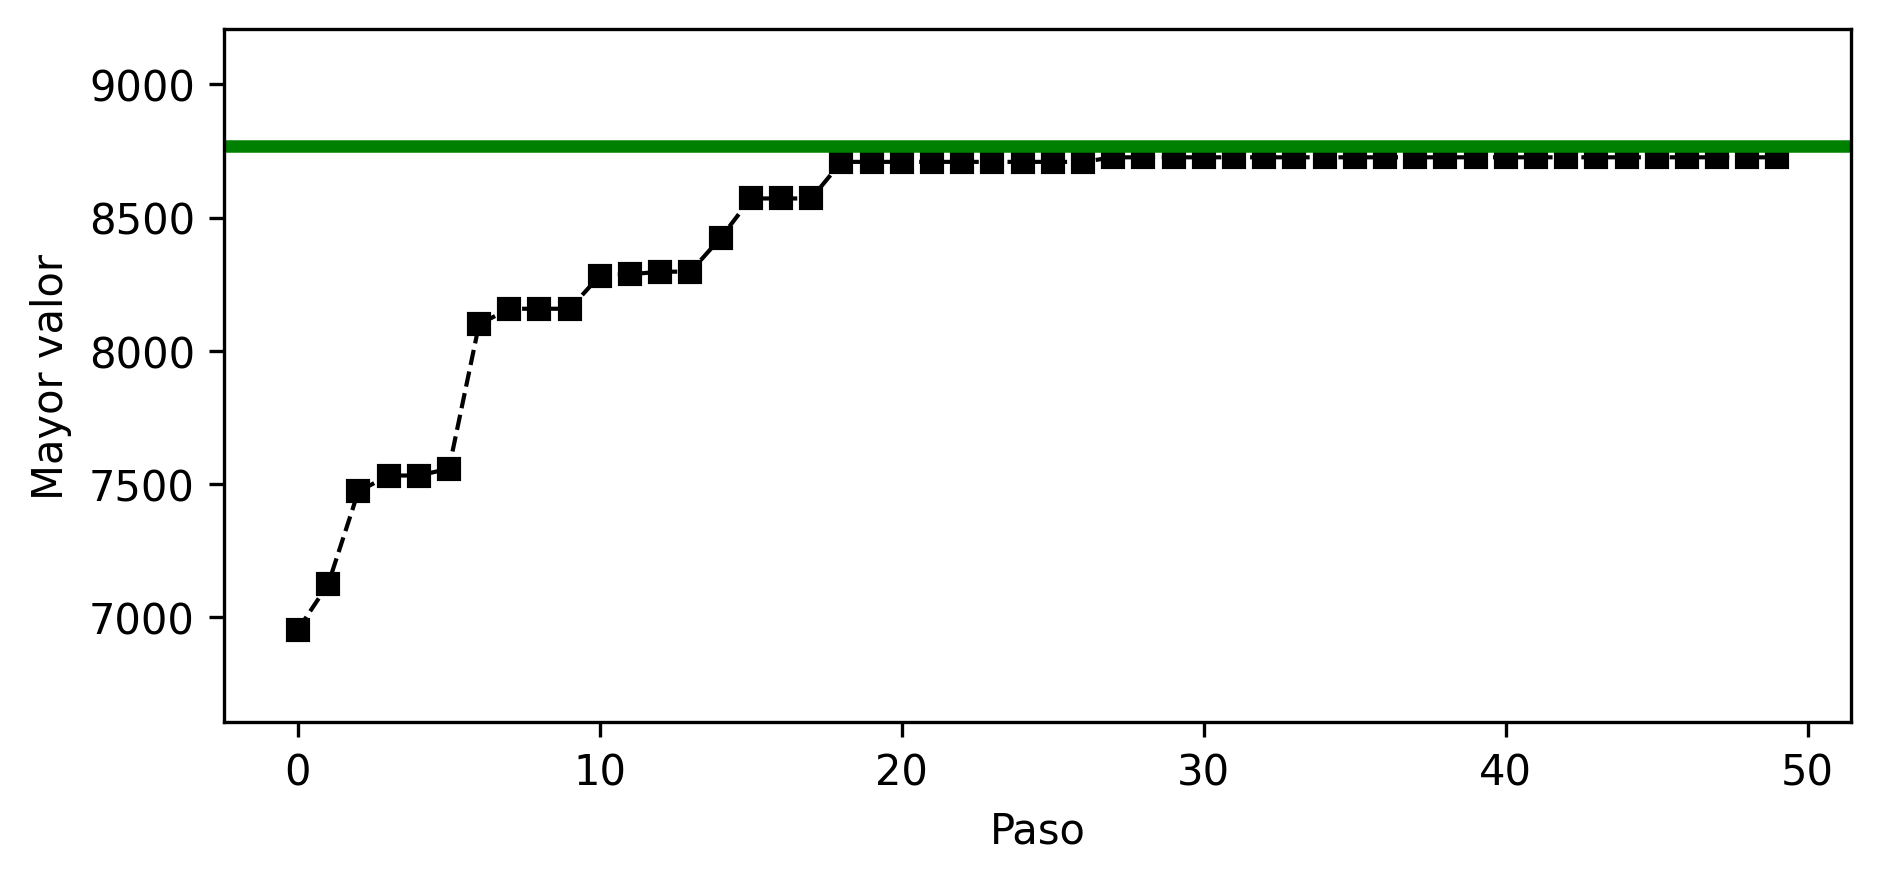
\includegraphics[width=\linewidth]{imagenes/figura_rp1.png}
\end{subfigure}
\caption{Grafica de comportamiento regla 2 .}
\label{fig:westminster}
\end{figure}
%%%%%%%%%%%%%%%%%%%%%%%  final 



%%%%%%%%%%%%%%%%%%%%% imagen 3
\begin{figure}[H]
\centering
\begin{subfigure}[b]{1.0\linewidth}
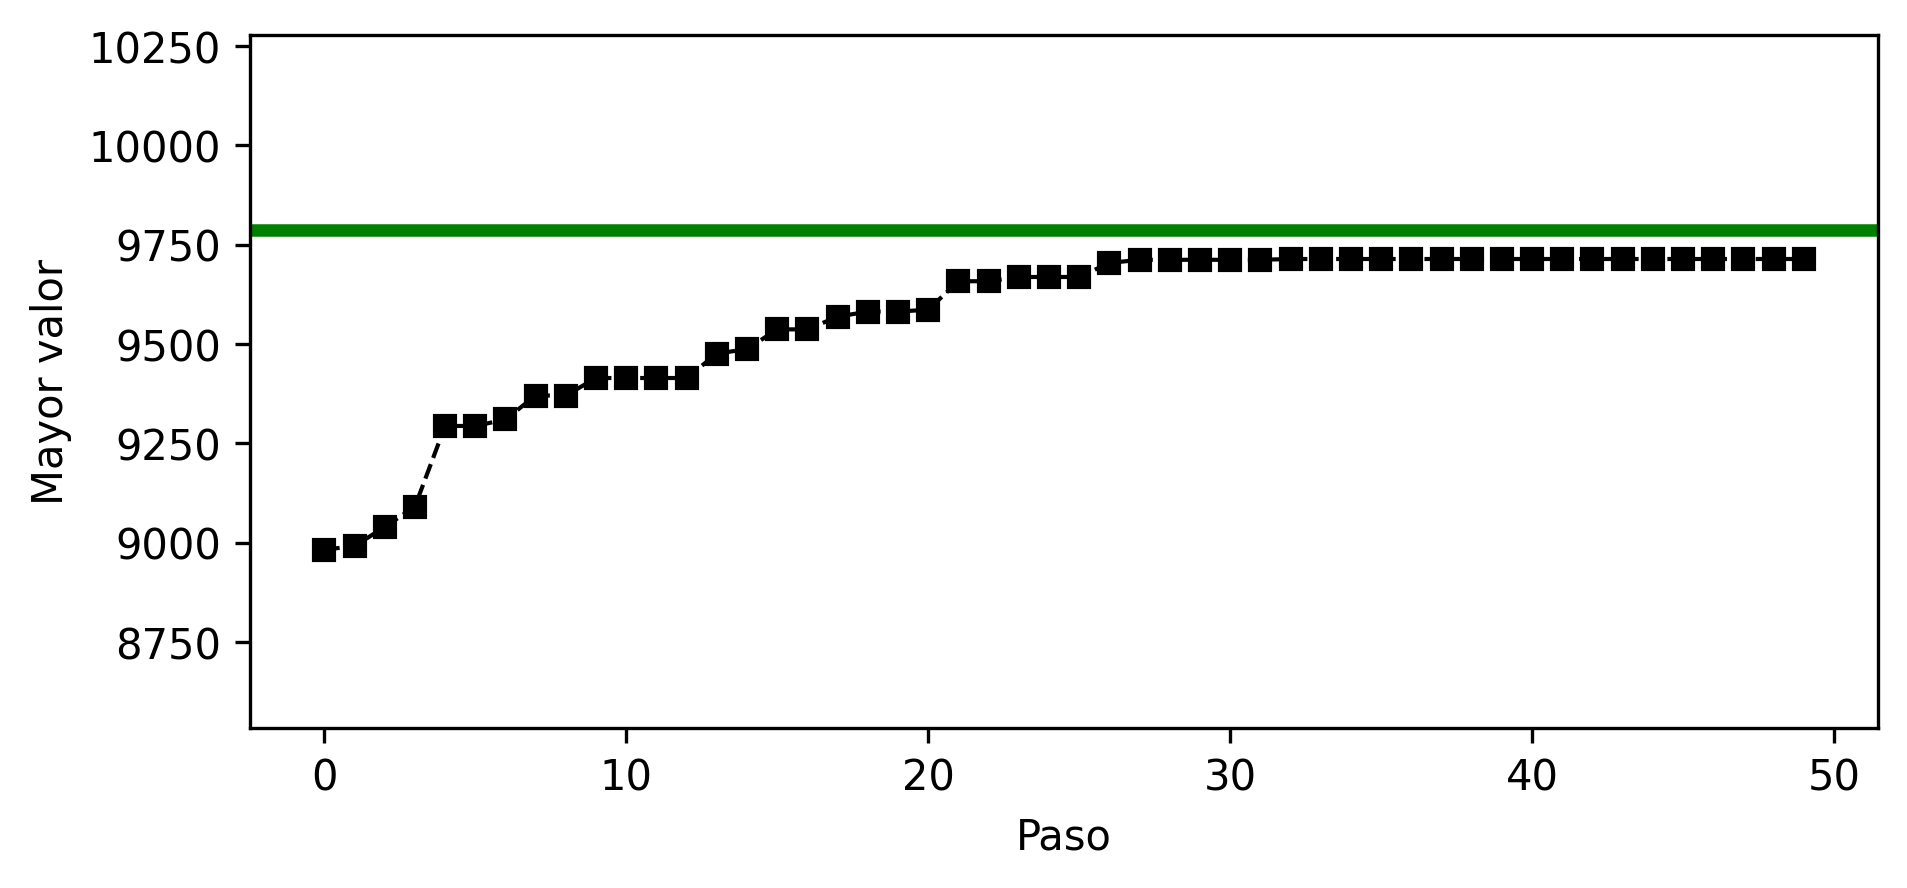
\includegraphics[width=\linewidth]{imagenes/figura_rp3.png}
\end{subfigure}
\caption{Grafica de comportamiento regla 3.}
\label{fig:westminster}
\end{figure}
%%%%%%%%%%%%%%%%%%%%%%%  final 
%%%%%%%%%%%%%%%%%%%%% imagen 4
\begin{figure}[H]
\centering
\begin{subfigure}[b]{1.0\linewidth}
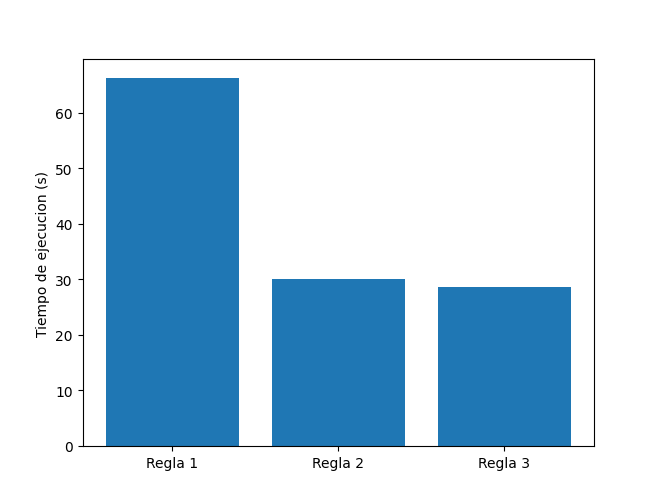
\includegraphics[width=\linewidth]{imagenes/figura_rp4.png}
\end{subfigure}
\caption{Gráfica de tiempo de ejecución.}
\label{fig:westminster}
\end{figure}
%%%%%%%%%%%%%%%%%%%%%%%  final 


%%%%%%%%%%%%%%%%%%%%% imagen 5
\begin{figure}[H]
\centering
\begin{subfigure}[b]{1.0\linewidth}
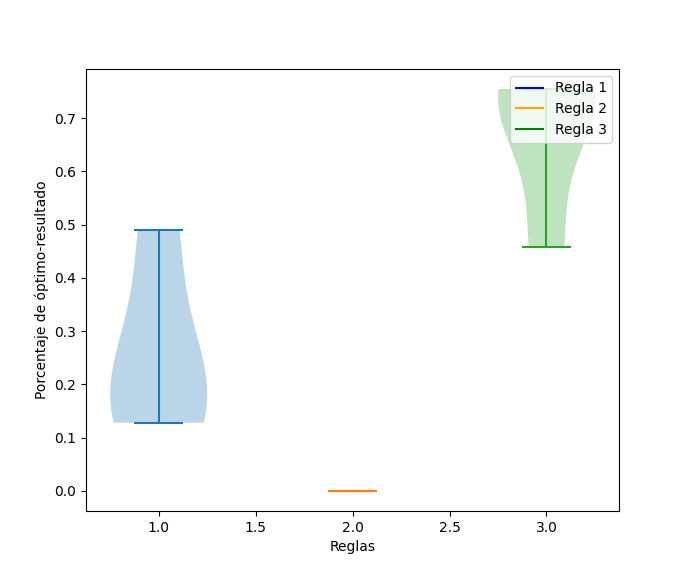
\includegraphics[width=\linewidth]{imagenes/figura_rp5.png}
\end{subfigure}
\caption{Grafica de Porcentaje.}
\label{fig:westminster}
\end{figure}
%%%%%%%%%%%%%%%%%%%%%%%  final 




 \section{Conclusión}
Se mostró con graficas de violín que con las instancias (0.5, 1000, 2000)es el que más se acerca al dato correcto pero las instancias que sobran se demostró que tienen mejor tiempo. 
.

 \bibliography{biblio.bib}
 \bibliographystyle{unsrtnat}

 \end{document}


